%%%%%%%%%%%%%%%%%%%%%%%%%%%%%%%%%%%%%%%%%%%%%%%%%%%%%%%%%%%%%%%%%%%
%TO AVOID FORMATTING ISSUES, COMPILE THIS ONLY AT WWW.OVERLEAF.COM%
%%%%%%%%%%%%%%%%%%%%%%%%%%%%%%%%%%%%%%%%%%%%%%%%%%%%%%%%%%%%%%%%%%%

%%%%%%%%%%%%%%%%%%%%%%%%%%%%%%%%%%%%%%%%%%%%%%%%%%%%%%%%%%%%%%%%%%%
\documentclass[a4paper,12pt]{article}
\usepackage{graphicx}
\usepackage{listings}
%To use this font, you need XeTex or LuaTex, prefer openleaf
\newenvironment{codefont}{\fontfamily{ccr}\selectfont}{\par}

\title{
	\normalfont \normalsize 
	\textsc{Pimpri Chinchwad College of Engineering \\ 
		Computer Laboratory - IV} \\
	[10pt] 
	\rule{\linewidth}{0.5pt} \\[6pt] 
	\huge Assignment No - A2 \\
	\rule{\linewidth}{2pt}  \\[10pt]
}
\author{}
\date{\normalsize}


\begin{document}
\maketitle

%%%%%%%%%%%%%%%%%%%%%%%
% FOR A NUMBERED LIST
% \begin{enumerate}
% \item Your_Item
% \end{enumerate}
%%%%%%%%%%%%%%%%%%%%%%%
% FOR A BULLETED LIST
% \begin{itemize}
% \item Your_Item
% \end{itemize}
%%%%%%%%%%%%%%%%%%%%%%%
% TO IMPORT AN IMAGE
% \includegraphics[width=\textwidth]{name_of_file}
% \textwidth makes the picture the width of the paragraphs
%%%%%%%%%%%%%%%%%%%%%%%%%%%%%%
% TO CREATE A FIGURE WITH A NUMBER AND CAPTION
% \begin{figure}
% \includegraphics[width=\textwidth]{image}
% \caption{Your Caption Goes Here}
% \label{your_label}
% \end{figure}
% REFER TO YOUR FIGURE LATER WITH
% \ref{your_label}
% LABELS NEED TO BE ONE WORD
%%%%%%%%%%%%%%%%%%%%%%%%%%%%%
% TO ADD CODE
% \begin{codefont}
% Some code in "courier" font
%\end{codefont}
%%%%%%%%%%%%%%%%%%%%%%%%%%%%%
\section{Aim : }
	\paragraph{} Using Divide and Conquer Strategies to design an efficient class for Concurrent Quick Sort and the input
	data is stored using XML. Use object oriented software design method and Modelio/ StarUML2.x Tool.
	Perform the efficiency comparison with any two software design methods. Use necessary USE-CASE
	diagrams and justify its use with the help of mathematical modeling. Implement the design using Scala/
	Python/Java/C++.
	
\section{Objective : }
	\begin{itemize}
		\item To study and implement Quick Sort  algorithm  concurrently.
		\item To use object oriented software design method.
		\item To design necessary UML diagrams.
	\end{itemize}
		
\section{Mathematical Model : }
	This problem can be mathematically modelled as follows,
	\newpage
		Consider a set S consisting of all the elements related to a program.The mathematical model is given as below,\\\\
		\textbf{S=\{s,e,X,Y,Fme\} }\\\\
		Where,\\
		\textbf{s} = Initial State\\
		\textbf{e} = End State\\
		\textbf{X} = Input. 
		\begin{itemize}
			\item  x=\{Unsorted Elements\} 
		\end{itemize}
		\textbf{Y} = Output. 
		\begin{itemize}
			\item y=\{Sorted Elements\} 
		\end{itemize}
		\textbf{Fme} = Algorithm \\\\
		int createPartition(int elements[], int begin, int end) \\
		\{\\
		int temp, temp1;\\
		int x = elements[end];\\
		int i = begin - 1;\\
		for(int j = begin; j<= end - 1; j++) {\\
			if(elements[j] <= x) {\\
				i = i+1;\\
				temp = elements[i];\\
				elements[i] = elements[j];\\
				elements[j] = temp;\\
				\}\\
				\}\\
				temp1 = elements[i + 1];\\
				elements[i + 1] = elements[end];\\
				elements[end] = temp1;\\
				return i + 1;\\
				\}\\
	
\section{Theory : }
	\subsection{Divide and Conquer strategy : }
		\begin{itemize}
			\item Given a function to compute on an inputs the divide and conquer strategy suggest splitting the input into k distinct input sets ,such that 1<k<n yielding k sub problems.
			
			\item These sub problems must be solved and then method must be found to combine the sub solution into a solution of a whole.
			
			\item If the sub problems are relatively large then the divide and conquer strategy can be reapplied.
			
			\item Often the sub problems are of the same type as the same original problem for which the reapplication of divide and conquer principle is naturally expressed by a recursive algorithm.
		\end{itemize}
		
	\subsection{Quick Sort Algorithm :}
		\subsubsection{Features of Quick Sort :}
			\begin{itemize}
				\item Similar to mergesort - divide-and-conquer recursive algorithm 
				\item One of the fastest sorting algorithms 
				\item Average running time O(NlogN) 
				\item Worst-case running time O(N2)
			\end{itemize}
		
		\subsubsection{Basic idea of Quick Sort :}
			\begin{enumerate}
				\item Pick one element in the array, which will be the pivot. 
				\item Make one pass through the array, called a partition step, re-arranging the entries so that: 
					\begin{itemize}
						\item the pivot is in its proper place. 
						\item entries smaller than the pivot are to the left of the pivot. 
						\item entries larger than the pivot are to its right. 
					\end{itemize}
				\item Recursively apply quicksort to the part of the array that is to the left of the pivot, and to the right part of the array. 
			\end{enumerate}
		
		\subsubsection{Algorithm : } We will dicuss the quicksort algorithm in detail,
		
		\begin{enumerate}
			\item Choosing the pivot \\ \textbf{ Choosing the pivot is an essential step.} Depending on the pivot the algorithm may run very fast, or in quadratic time.:
			\begin{enumerate}
				\item  Some fixed element: e.g. the first, the last, the one in the middle,this is a bad choice - the pivot may turn to be the smallest or the largest element, then one of the partitions will be empty.
				\item Randomly chosen (by random generator ) - still a bad choice. 
				\item The median of the array (if the array has N numbers, the median is the [N/2] largest number. This is difficult to compute - increases the complexity. 
				\item The median-of-three choice: take the first, the last and the middle element. Choose the median of these three elements. \\
				
				\textbf{Example:}\\
				8, 3, 25, 6, 10, 17, 1, 2, 18, 5 \\
				The first element is 8, the middle - 10, the last - 5. \\
				The median of [8, 10, 5] is 8
			\end{enumerate}
			
			\item Partitioning \\ \textbf{Partitioning is illustrated on the above example.}
			\begin{enumerate}
				\item The first action is to get the pivot out of the way - swap it with the last element \\
				5, 3, 25, 6, 10, 17, 1, 2, 18, 8\\
				\item  We want larger elements to go to the right and smaller elements to go to the left.Two "fingers" are used to scan the elements from left to right and from right to left:\\
				
				[5, 3, 25, 6, 10, 17, 1, 2, 18, 8]\\
				\^\qquad\qquad\qquad\qquad\qquad\qquad\^\\
				i \qquad\qquad\qquad\qquad\qquad\qquad j\\
				\begin{enumerate}
					\item  While i is to the left of j, we move i right, skipping all the elements less than the pivot. If an element is found greater then the pivot, i stops
					\item  While j is to the right of i, we move j left, skipping all the elements greater than the pivot. If an element is found less then the pivot, j stops
					\item  When both i and j have stopped, the elements are swapped.
					\item  When i and j have crossed, no swap is performed, scanning stops, and the element pointed to by i is swapped with the pivot .In the example the first swapping will be between 25 and 2, the second between 10 and 1.
				\end{enumerate}
				\item Restore the pivot.
				After restoring the pivot we obtain the following partitioning into three groups:\\
				$[5, 3, 2, 6, 1] [ 8 ] [10, 25, 18, 17]$		
			\end{enumerate}	
			\item Recursively quick sort the left and the right parts
		\end{enumerate} 


	
	\subsection{Software Functions : }
		Here is the function, that implements the partitioning.\\
		left points to the first element in the array currently processed, right points to the last element. \\
		\lstset{language=C}          
		\begin{lstlisting}[frame=single] 
if( left + 10 $<$= right)
{
int i = left, j = right - 1;
for ( ; ; )
{
while (a[++i] $<$ pivot  ) {}  // move the left finger
while (pivot  $<$ a[--j] ) {}  // move the right finger
if (i $<$ j) swap (a[i],a[j]);  // swap       
else  break;     // break if fingers have crossed
}
swap (a[I], a[right-1);   // restore the pivot
quicksort ( a, left, i-1);  // call quicksort for the 
                            //left part
quicksort (a, i+1, right);// call quicksort for the 
                          //left part
}
else 
insertionsort (a, left, right);
		\end{lstlisting}
		If the elements are less than 10, quicksort is not very efficient. 
		Instead insertion sort is used at the last phase of sorting.
		
		\subsubsection{Implementation notes:}
		Compare the two versions:
		\begin{enumerate}
			
			\item[A.] 
			while (a[++i] $<$ pivot) {}
			while (pivot $<$ a[--j]) {}
			
			if (i $<$ j) swap (a[i], a[j]);
			else break;
			\item[B.] 
			
			while (a[i] $<$ pivot) {i++;}
			while (pivot $<$ a[j] ) {j--;}
			
			if (i $<$ j) swap (a[i], a[j]);
			else break;
		\end{enumerate}
		If we have an array of equal elements, the second code will never increment i or decrement j, 
		and will do infinite swaps. i and j will never cross.

		
	\subsection{Concurrency in Quick sort : }
		\textbf{Concurrent Quicksort} \\
		\par	Simple concurrent implementation uses a collection of worker threads and a coordinator thread.The coordinator sends a message to an idle worker telling it to sort the array and waits to receive messages from the workers about the progress of the algorithm. \par
		A worker partitions a sub-array, and every time that worker gets ready to call the partition routine on a smaller array, it checks to see if there is an idle worker to assign the work to. If so, it sends a message to the worker to start working on the sub-problem; if not the current worker makes calls the partition routine itself.
		\par	After each partitioning, two recursive calls are (usually) made, so there are plenty of chances to start other workers.The diagram below shows two workers sorting the same 5-element array. Each blue line represents the flow of control of a worker thread, and the red arrow represents the message sent from one worker to start the other. (Since the workers proceed working concurrently, it is no longer guaranteed that the smaller elements in the array will be ordered before the larger; what is certain is that the two workers will never try to manipulate the same elements.)
		\par	A worker can complete working either because it has directly completed all the work sorting the subarray it was initially called on, or because it has ordered a subset of that array but has passed some or all of the remaining work to other workers.In either case, it reports the number of elements it has ordered back to the coordinator.(The number of elements a worker has ordered is the number of partitions of sub-arrays that have 1 or more members).
		\par	When the coordinator hears that all the elements in the array have been ordered, it tells the workers that there is nothing left to do, and the workers exit. That’s the basic idea.\\\\
		\textbf{Multithreading in C++ :}\\
		\textbf{Demo Example:} \\
		Create a function that you want the thread to execute. I'll demonstrate with a trivial example:\\
		void task1(std::string msg)\\
		\{\ \\
			std::cout $<<$ $"$task1 says: $"$ $<<$ msg; \\
		\}\\\
		Now create the thread object that will ultimately invoke the function above like so:
		std::thread t1(task1, "Hello");\\
		( You need to \#include $<$thread$>$ to access the std::thread class )\\
		As you can see, the constructor's arguments are the function the thread will execute, followed by the function's parameters.\\
		Finally, join it to your main thread of execution like so:\\
		t1.join(); \\
		(Joining means that the thread who invoked the new thread will wait for the new thread to finish execution, before it will continue it's own execution).\\	
			
\section{Testing}
\subsection{BLACK BOX TESTING : }
		 Black-box testing is a method of software testing that examines the functionality of an application based on the specifications. It is also known as Specifications based testing. Independent Testing Team usually performs this type of testing during the software testing life cycle.This method of test can be applied to each and every level of software testing such as unit, integration, system and acceptance testing.\\
		 Black box testing techniques are :\\
1) Equivalence Class Partitioning\\
2) Boundary Value Analysis\\
3) Decision Tables\\
4) State Transition Diagrams (or) State Transition Diagrams\\
5) Orthogonal Arrays\\
6) All Pairs Technique\\

\subsection{WHITE BOX TESTING :}
		 White Box Testing (WBT) is also known as Code-Based Testing or Structural Testing. White box testing is the software testing method in which internal structure is being known to tester who is going to test the software.In this method of testing the testcases are calculated based on analysis internal structure of the system based on Code coverage, branches coverage, paths coverage, condition Coverage etc. Typically such method are used at Unit Testing of the code but this different as Unit testing done by the developer \& White Box Testing done by the testers, this is learning the part of the code \& finding out the weakness in the software program under test.
For tester to test the software application under test is like a white/transparent box where the inside of the box is clearly seen to the tester (as tester is aware/access of the internal structure of the code), so this method is called as White Box Testing.

The White-box testing is one of the best method to find out the errors in the software application in early stage of software development life cycle. In this process the deriving the test cases is most important part. The test case design strategy include such that all lines of the source code will be executed at least once or all available functions are executed to complete 100 percent  code coverage of testing. For this, we will use Flow Graphs. Flow graphs are, Syntactic abstraction of source code Resembling to classical flow charts Forms the basis for white box test case generation principles.Conventions of flow graph notation. \\
Why and When White-Box Testing:\\
White box testing is mainly used for detecting logical errors in the program code. It is used for
debugging a code, finding random typographical errors, and uncovering incorrect programming
assumptions .
White box testing is done at low level design and implementable code. It can be applied at all levels of
system development especially Unit, system and integration testing. White box testing can be used for
other development artefacts like requirements analysis, designing and test cases .
White box testing techniques are:\\
1. Static white box testing\\
a. Desk checking\\
b. Code walkthrough\\
c. Formal Inspections\\
2. Structural White box testing\\
a. Control flow/ Coverage testing\\
b. Basic path testing\\
c. Loop testing\\
d. Data flow \\


	\begin{figure}[h!]
		\centering
		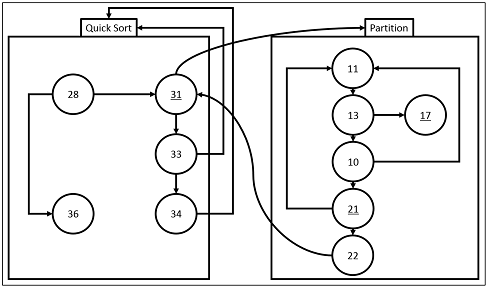
\includegraphics[scale=0.80]{graph.png}
		\caption{Flow Graph}
		\label{Flow Graph}
	\end{figure}

	\begin{figure}[h!]
		\centering
		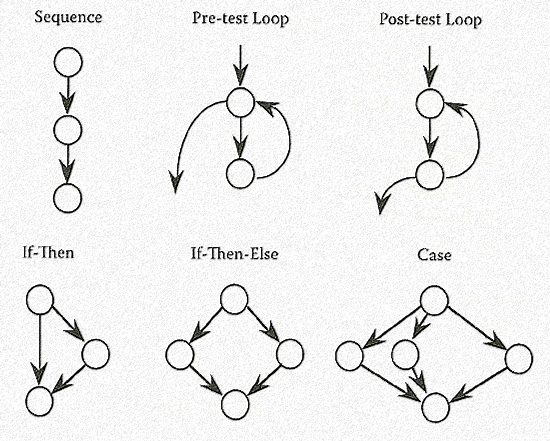
\includegraphics[scale=0.50]{flowgraph.png}
		\caption{Flow Graph Notation}
		\label{Flow Graph Notation}
	\end{figure}

	\newpage
	\subsection{Class Diagram}
	\begin{figure}[h!]
		\centering
		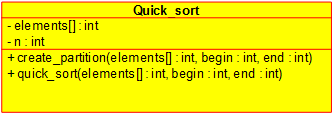
\includegraphics[scale=0.80]{quick-sort-class}
		\caption{Class Diagram}
		\label{Flow Graph}
	\end{figure}
	
	\subsection{Use Case}
	\begin{figure}[h!]
		\centering
		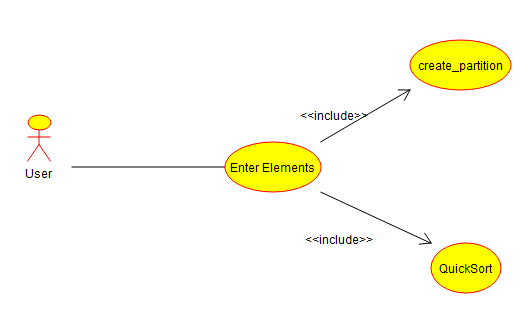
\includegraphics[scale=0.80]{quick-sort-use}
		\caption{Use Case Diagram}
		\label{Use Case}
	\end{figure}
	\subsection{ POSITIVE/NEGATIVE TESTING }


\textbf{Example:}\\
Sample Input: For integer array\\
int A[] = f21; 33; 67; 72; 27; 10; 2; 66; 81; 1g; Function is passed following arguments:\\
quickSort(A; 0; 9);\\
Output obtained:\\
New partition: Low=0 High=9\\
Swapped 21 with Pivot 1\\
New partition: Low=1 High=9\\
Swapped 33 with 10\\
Swapped 67 with 2\\
Swapped 72 with Pivot 21\\
New partition: Low=1 High=2\\
Swapped 10 with Pivot 2\\
New partition: Low=4 High=9\\
Swapped 27 with 27\\
Swapped 33 with 33\\
Swapped 67 with 67\\
Swapped 66 with 66\\
Swapped 81 with Pivot 72\\
New partition: Low=4 High=7\\
Swapped 27 with 27\\
Swapped 33 with 33\\
Swapped 67 with Pivot 66\\
New partition: Low=4 High=5\\
Swapped 27 with 27\\
Swapped 33 with Pivot 33\\
1,2,10,21,27,33,66,67,72,81,\\
Note:\\
The underlined nodes are the ones being tested. The above output shows that every test region is
covered for given input.\\
\newpage

\textbf{Positive Testing :}\\
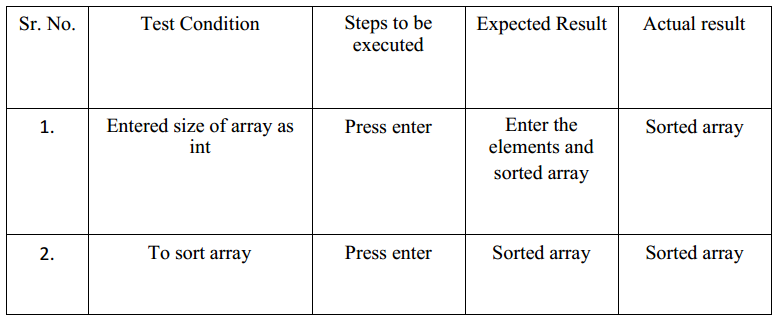
\includegraphics[width=\textwidth]{quicksort_positive}
\vspace{30px}

\textbf{Negative Testing :}\\
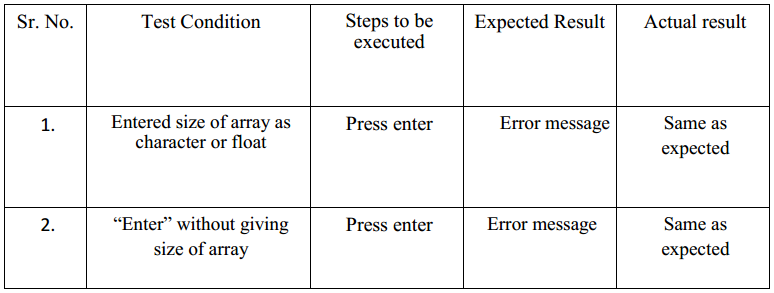
\includegraphics[width=\textwidth]{quicksort_negative}



\section{Conclusion : }
	\paragraph{} We have succesfully implemented quick sort concurrently, using divide and conquer strategy, we have  used object oriented software design method and Modelio Tool
\vspace{20px}
\begin{center}
	\begin{tabular}
		{|c|c|c|c|}\hline
		{\bf Roll No.}		&{\bf Name of Student}		&{\bf Date of Performance}  				&{\bf Date of Submission}  \\ \hline
		{302}	&	{Abhinav Bakshi}& 	{21/12/15}	&  {04/01/16} \\ \hline
	\end{tabular}\\ 
\end{center}
\newpage
\section{Plagarism Report}
		\begin{figure}[h!]
		\centering
		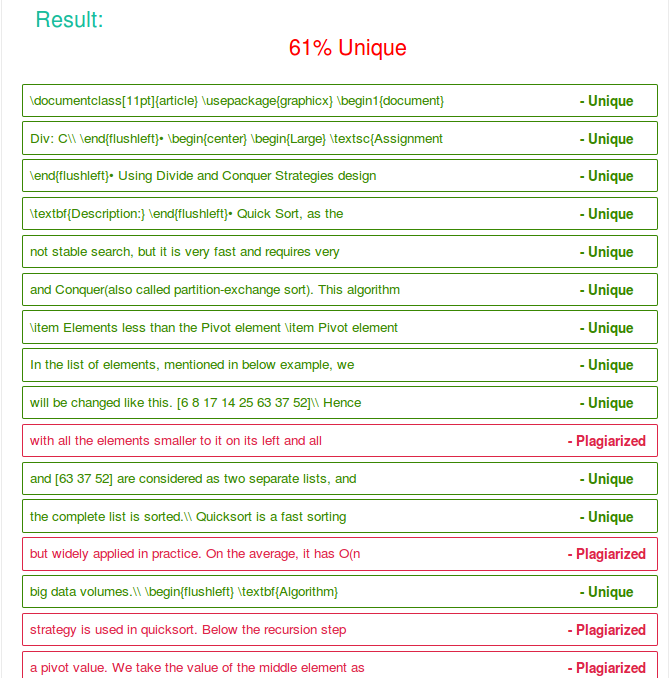
\includegraphics[scale=0.80]{Quick_Sort_Plag.png}
		\caption{Plagarism Report}
		\label{Plagarism Report}
	\end{figure}
\end{document}
 

 
